\documentclass[12pt,a4paper,oneside]{report}

\usepackage[margin=1in,headheight=22pt,headsep=0.28in]{geometry}
\usepackage[T1]{fontenc}
\usepackage[utf8]{inputenc}
\usepackage{lmodern}
\usepackage{microtype}
\usepackage{booktabs}
\usepackage{array}
\usepackage{longtable}
\usepackage{tabularx}
\usepackage{multirow}
\usepackage{enumitem}
\usepackage[table]{xcolor}
\usepackage{xurl}
\usepackage{hyperref}
\usepackage{listings}
\usepackage{amsmath}
\usepackage{amssymb}
\usepackage{graphicx}
\usepackage{float}
\usepackage{placeins}
\usepackage{needspace}
\usepackage[font=small,labelfont=bf]{caption}
\usepackage{subcaption}
\usepackage{fancyhdr}
\usepackage{titlesec}
\usepackage{chngcntr}
\usepackage{tocloft}
\usepackage{etoolbox}

\definecolor{covergreen}{RGB}{35,107,72}
\definecolor{accentgreen}{RGB}{224,239,228}
\definecolor{warningyellow}{RGB}{252,244,210}

\hypersetup{
  colorlinks=true,
  linkcolor=blue!45!black,
  citecolor=blue!45!black,
  urlcolor=blue!45!black,
  pdftitle={Accelera: Graph-Based ML Pipelines, Benchmarking, and Multi-Target Model Deployment},
  pdfauthor={Mazen Adel}
}

\setlength{\parindent}{0.18in}
\setlength{\parskip}{0.15em}

\titleformat{\chapter}[hang]
  {\normalfont\bfseries\fontsize{22}{26}\selectfont\raggedright}
  {\chaptername\ \thechapter:}{0.5em}{}
\titleformat{name=\chapter,numberless}[hang]
  {\normalfont\bfseries\fontsize{22}{26}\selectfont}{}{0pt}{}
\titlespacing*{\chapter}{0pt}{0pt}{18pt}
\titleformat{\section}
  {\normalfont\bfseries\fontsize{16}{20}\selectfont}
  {\thesection}{0.6em}{}
\titlespacing*{\section}{0pt}{15pt}{7pt}
\titleformat{\subsection}
  {\normalfont\bfseries\fontsize{13}{16}\selectfont}
  {\thesubsection}{0.6em}{}
\titlespacing*{\subsection}{0pt}{11pt}{5pt}

\pagestyle{fancy}
\fancyhf{}
\fancyhead[R]{\textbf{Accelera} \textcolor{covergreen}{2026}}
\fancyfoot[R]{\thepage\,|\,Page}
\renewcommand{\headrulewidth}{0.5pt}
\renewcommand{\footrulewidth}{0.3pt}
\fancypagestyle{plain}{\pagestyle{fancy}}

\counterwithin{figure}{chapter}
\counterwithin{table}{chapter}
\renewcommand{\lstlistingname}{Algorithm}
\renewcommand{\lstlistlistingname}{List of Algorithms}
\setlength{\emergencystretch}{2em}
\raggedbottom

\lstdefinestyle{paperpython}{
  basicstyle=\ttfamily\footnotesize,
  breaklines=true,
  frame=single,
  columns=fullflexible,
  keepspaces=true,
  showstringspaces=false,
  keywordstyle=\color{blue!55!black},
  commentstyle=\color{green!35!black}
}

\lstdefinestyle{algostyle}{
  basicstyle=\rmfamily\scriptsize,
  backgroundcolor=\color{white},
  frame=tb,
  rulecolor=\color{black},
  framerule=0.45pt,
  framesep=3pt,
  xleftmargin=0pt,
  xrightmargin=0pt,
  numbers=left,
  numberstyle=\scriptsize\rmfamily,
  numbersep=5pt,
  columns=fullflexible,
  keepspaces=true,
  showstringspaces=false,
  breaklines=true,
  breakatwhitespace=false,
  breakautoindent=false,
  breakindent=0pt,
  captionpos=t,
  aboveskip=0.8em,
  belowskip=0.8em
}

\lstset{style=paperpython}
\renewcommand{\thelstnumber}{\arabic{lstnumber}:}

\newcommand{\systemname}{Accelera}
\newcommand{\modulepath}[1]{\texttt{#1}}
\newcommand{\todoitem}[1]{\textcolor{red!65!black}{[TODO: #1]}}

\begin{document}

% -----------------------------------------------------------------------------
% TITLE PAGE
% -----------------------------------------------------------------------------
\begin{titlepage}
\thispagestyle{empty}
\begin{center}


\includegraphics[width=0.12\textwidth]{../imgs/CU_logo.png}\\
{\fontsize{12}{14}\selectfont Cairo University}\\
{\fontsize{12}{14}\selectfont Faculty of Engineering}\\
{\fontsize{12}{14}\selectfont Department of Computer Engineering}\\

\vspace{0.8cm}

{\bfseries\fontsize{22}{26}\selectfont Accelera: Graph-Based ML Pipelines, Benchmarking Platform, and Multi-Target Model Deployment}

\vspace{0.35cm}

{\fontsize{16}{20}\selectfont Pipeline Parallelism, Web-Based Leaderboards, and Containerized Deployments}

\vspace{0.8cm}


\includegraphics[width=0.22\textwidth]{../imgs/accelera.png}

\vspace{0.7cm}

{\fontsize{12}{14}\selectfont
A Graduation Project Individual Report Submitted\\
to\\[0.15cm]
Faculty of Engineering, Cairo University\\[0.15cm]
in Partial Fulfillment of the Requirements for the Degree\\[0.15cm]
of\\[0.15cm]
Bachelor of Science in Computer Engineering.
}

\vspace{0.8cm}

{\bfseries\fontsize{16}{18}\selectfont Presented by}

\vspace{0.25cm}

{\fontsize{14}{16}\selectfont Mazen Adel}\\[0.15cm]
{\fontsize{12}{14}\selectfont Student ID: 9220625}

\vspace{0.6cm}

{\bfseries\fontsize{16}{18}\selectfont Supervised by}

\vspace{0.25cm}

{\fontsize{14}{16}\selectfont Dr. Salma Abdel Monem}

\vspace{0.45cm}

{\fontsize{12}{14}\selectfont June 2026}

\vfill

{\fontsize{11}{14}\selectfont
All rights reserved. This report may not be reproduced in whole or in part,
by photocopying or other means, without the permission of the author or department.
}

\end{center}
\end{titlepage}

% -----------------------------------------------------------------------------
% ABSTRACT
% -----------------------------------------------------------------------------
\pagenumbering{arabic}
\setcounter{page}{2}

\begin{abstract}
This report details the individual design, implementation, and verification of three core modules in the \systemname{} framework: the Pipeline Module (graph execution and parallelism), the Benchmark Module (REST API, authentication, dashboards, and automated scoring), and the Deployment Module (multi-target deployment, runtime schema validation, telemetry logging, and model version control). 

Within the Pipeline Module, Mazen implemented the C++ back-end execution engine supporting branching workflows, topological sorting, DAG constraints, and duplicate-node optimization. Specifically, this work presents his implementation of a thread-safe parallel scheduler using counting semaphores that executes independent branches concurrently while releasing consumed intermediate buffers to minimize peak memory usage, alongside a native Merge Node implementing class and probability-based majority voting strategies.

Within the Benchmark Module, Mazen developed a Node.js REST API using Express and MongoDB to handle secure user authentication (JWT and bcrypt), dataset uploads, leaderboard management, and validation of submitted predictions against hidden ground truths. He also built a React frontend consisting of dedicated User and Admin Dashboards for task filtering, leaderboard viewing, and administrator-level user management.

Finally, the Deployment Module forms the main contribution of this individual work. It integrates a production-ready FastAPI web server featuring runtime data validation via Great Expectations, an asynchronous request tracking and telemetry logging database, a lightweight model Version Control System (VCS) with SHA-1 hash commits and automatic rollback, and an automated deployment engine targeting Local Docker, Heroku, and remote AWS EC2 instances over SSH.
\end{abstract}

% -----------------------------------------------------------------------------
% TABLES OF CONTENTS & LISTS
% -----------------------------------------------------------------------------
\tableofcontents
\listoffigures
\listoftables
\clearpage

% -----------------------------------------------------------------------------
% CHAPTER 1: INTRODUCTION
% -----------------------------------------------------------------------------
\chapter{Introduction}
\label{chap:introduction}

\section{Project Context and Goals}
Developing and deploying machine learning pipelines in professional settings requires solving challenges that span different parts of the software lifecycle. A simple, linear script is often sufficient for training a single model on a local workstation. However, a production-grade machine learning system must evaluate multiple models, preprocessing methods, and hyperparameters, run experiments fairly, track version histories, and host models in scalable environments.

\systemname{} addresses these challenges by organizing the workflow into separate but integrated modules. This individual work focuses on three essential layers:
\begin{enumerate}
    \item \textbf{The Execution Layer (Pipeline Module):} Runs multi-branch pipelines efficiently on multi-core machines, handling dependencies, branching, merging, and memory management.
    \item \textbf{The Collaboration Layer (Benchmark Module):} Provides a central, secure platform where different developers can test their models on the same datasets under the same evaluation metrics.
    \item \textbf{The Serving Layer (Deployment Module):} Acts as the main focus of this work, responsible for packaging trained models, validating input data, saving prediction histories, and pushing services to container platforms.
\end{enumerate}

\section{Mazen Adel's Contributions}
As part of the \systemname{} development team, the author designed, implemented, and verified the following components:
\begin{itemize}[leftmargin=*]
    \item \textbf{Pipeline Module:} Developed the native C++ \modulepath{MergeNode} class and voting algorithms. Built the concurrent graph runner (\modulepath{runParallel}) using semaphores, GIL management, and memory optimizations.
    \item \textbf{Benchmark Module:} Programmed the Node.js Express backend and MongoDB schemas for users, benchmarks, and submissions. Designed the React dashboards for users and administrators.
    \item \textbf{Deployment Module:} Designed and built the complete model serving system, which includes the FastAPI server, Uvicorn server, Great Expectations validation layer, telemetry logger, and CLI deployment tools for Docker, Heroku, and AWS EC2. Created the custom Model Version Control (VCS) subsystem.
\end{itemize}

\section{Report Organization}
The rest of this report is organized as follows: Chapter~\ref{chap:literature-survey} reviews the relevant background and related technologies. Chapter~\ref{chap:system-design} describes the architecture, schemas, and design constraints of the three modules. Chapter~\ref{chap:methodology} explains the details of the implementation and algorithms. Chapter~\ref{chap:verification} presents the testing results and verification, and Chapter~\ref{chap:conclusion} concludes with future improvements.

% -----------------------------------------------------------------------------
% CHAPTER 2: LITERATURE SURVEY
% -----------------------------------------------------------------------------
\chapter{Literature Survey}
\label{chap:literature-survey}

\section{Machine Learning Pipeline Abstractions}
Machine learning pipelines are commonly used to organize workflows. The most popular pipeline system is the linear model in \modulepath{scikit-learn}, which chains transformers and estimators together. However, a linear pipeline cannot naturally represent complex, non-linear workflows. For example, if a developer wants to compare three scaling methods and two classifiers, a linear system requires building six separate pipelines. This duplicates both code and execution time, as early steps must run repeatedly. Modern systems address this by representing workflows as Directed Acyclic Graphs (DAGs), where nodes represent computational steps and edges represent data dependencies.

\section{Automatic Concurrency and GIL Release}
In Python-based frameworks, running pipelines concurrently is limited by the Global Interpreter Lock (GIL). The GIL prevents multiple threads from executing Python bytecodes at the same time. To achieve true parallel execution on multi-core systems, heavy computations must be offloaded to compiled native languages like C++ using binding tools like \modulepath{pybind11}. When executing C++ code, the Python GIL can be released (\modulepath{py::gil\_scoped\_release}), allowing separate native threads to run independently on different CPU cores.

\section{Web Serving and Data Quality Layers}
Model serving requires turning saved binaries (such as pickle files) into active web endpoints. FastAPI is a common choice for this, utilizing asynchronous loops to handle concurrent requests. However, raw inputs submitted by users can contain invalid formats or values that cause models to crash. Data validation tools like Great Expectations help prevent this. They define schema rules (such as expected columns, types, and range boundaries) to check data quality at runtime before sending inputs to the model.

\section{Multi-Target Deployment Platforms}
Deploying serving containers involves different target architectures:
\begin{itemize}[leftmargin=*]
    \item \textbf{Local Docker:} Provides local isolation, ensuring the service runs identically in development and production.
    \item \textbf{Heroku Container Registry:} Simplifies cloud hosting by managing HTTP routing and container scaling automatically.
    \item \textbf{AWS EC2:} Offers raw virtual machines in the cloud, requiring custom SSH management, codebase synchronization, remote container building, and manual firewall configuration.
\end{itemize}

% -----------------------------------------------------------------------------
% CHAPTER 3: SYSTEM DESIGN AND ARCHITECTURE
% -----------------------------------------------------------------------------
\chapter{System Design and Architecture}
\label{chap:system-design}

\section{Pipeline Module Architecture}
The Pipeline Module represents machine learning workflows as a DAG. Nodes are split into six functional categories: input, preprocessing, model, prediction, metric, and merge. The DAG is compiled by sorting the nodes topologically, which ensures that parent nodes execute before their child nodes.

Two major optimizations were introduced by Mazen to improve execution performance:
\begin{enumerate}
    \item \textbf{Duplicate first-node sharing:} When multiple branches start with the same preprocessing step, the engine automatically shares the output of the first node rather than duplicating the calculation (Figures~\ref{fig:before_sharing} and \ref{fig:after_sharing}).
    \item \textbf{Active consumer counting:} The engine counts the active downstream consumers for each intermediate array. Once all child nodes finish execution, the parent node's temporary data is freed from RAM.
\end{enumerate}

\begin{figure}[H]
\centering
\begin{subfigure}{0.48\textwidth}
    \centering
    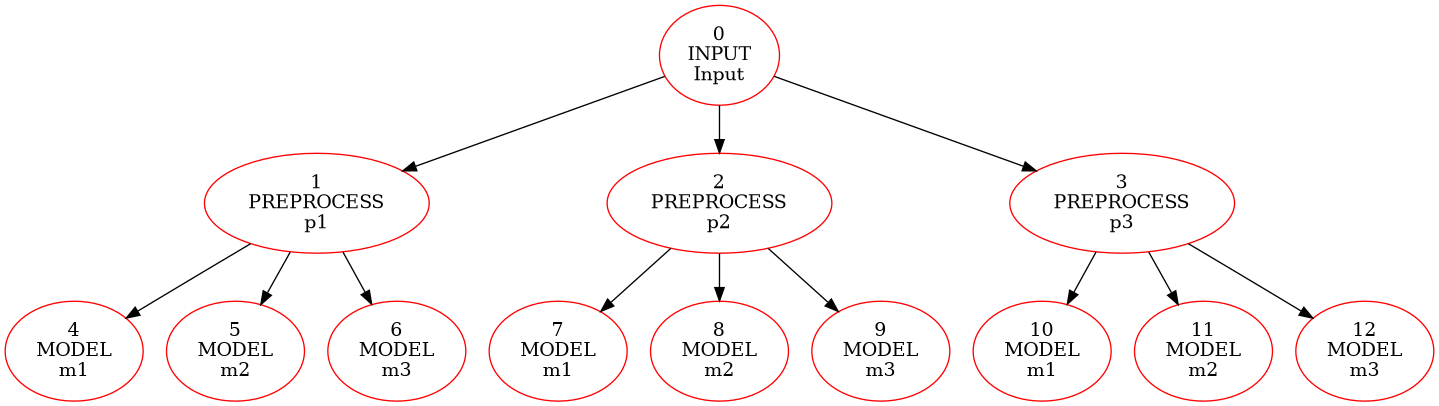
\includegraphics[width=\textwidth]{../imgs/before_sharing.png}
    \caption{Before duplicate sharing}
    \label{fig:before_sharing}
\end{subfigure}
\hfill
\begin{subfigure}{0.48\textwidth}
    \centering
    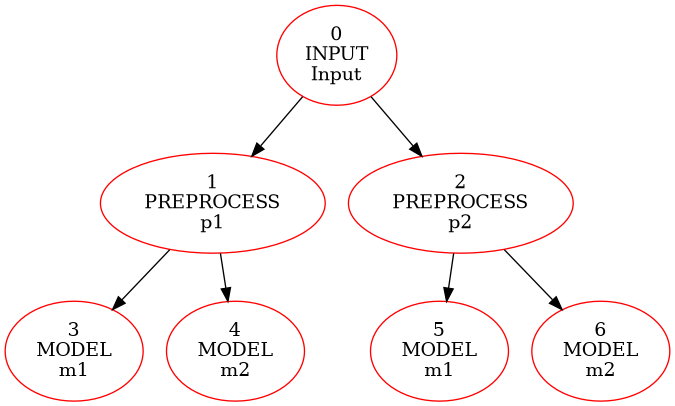
\includegraphics[width=\textwidth]{../imgs/after_sharing.png}
    \caption{After duplicate sharing}
    \label{fig:after_sharing}
\end{subfigure}
\caption{Optimization of Duplicate Node Sharing in DAGs}
\end{figure}

\section{Benchmark Module Architecture}
The Benchmark Module provides a web-based platform for comparing model performances. It consists of a React frontend and a Node.js backend using Express and MongoDB.

\subsection{Database Schema Design}
The database schemas are defined using Mongoose. The three main schemas are:
\begin{itemize}[leftmargin=*]
    \item \textbf{User Schema:} Stores names, emails, hashed passwords (via bcrypt), and role properties (\texttt{"user"} or \texttt{"admin"}).
    \item \textbf{Benchmark Schema:} Defines the title, description, target column name, problem type, Google Drive dataset links, and a reference to the evaluation metric schema.
    \item \textbf{Submission Schema:} Tracks the submitted repository link, predictions file link, submission date, and calculated score.
\end{itemize}

\subsection{Dashboard Views}
The User Dashboard lists active benchmarks and submissions. The Admin Dashboard is restricted to administrative users (Figure~\ref{fig:admin_dashboard_logic}), allowing them to browse and delete users, manage roles, and register new evaluation metrics.

\begin{figure}[H]
\centering
\begin{minipage}{0.65\textwidth}
\small
\renewcommand{\arraystretch}{1.15}
\begin{tabular}{|l|l|p{3.5cm}|}
\hline
\textbf{Role} & \textbf{Dashboard Access} & \textbf{Authorized Operations} \\ \hline
\texttt{user} & User Dashboard & View leaderboards, create benchmarks, submit predictions \\ \hline
\texttt{admin} & Admin Dashboard & View users, delete users, register new metrics \\ \hline
\end{tabular}
\end{minipage}
\caption{Access Control matrix for dashboards}
\label{fig:admin_dashboard_logic}
\end{figure}

\section{Deployment Module Architecture}
The Deployment Module is the primary contribution of this work. It packages trained estimators and preprocessors into a containerized REST service. Figure~\ref{fig:serving_architecture} outlines the serving and validation components.

\begin{figure}[H]
\centering
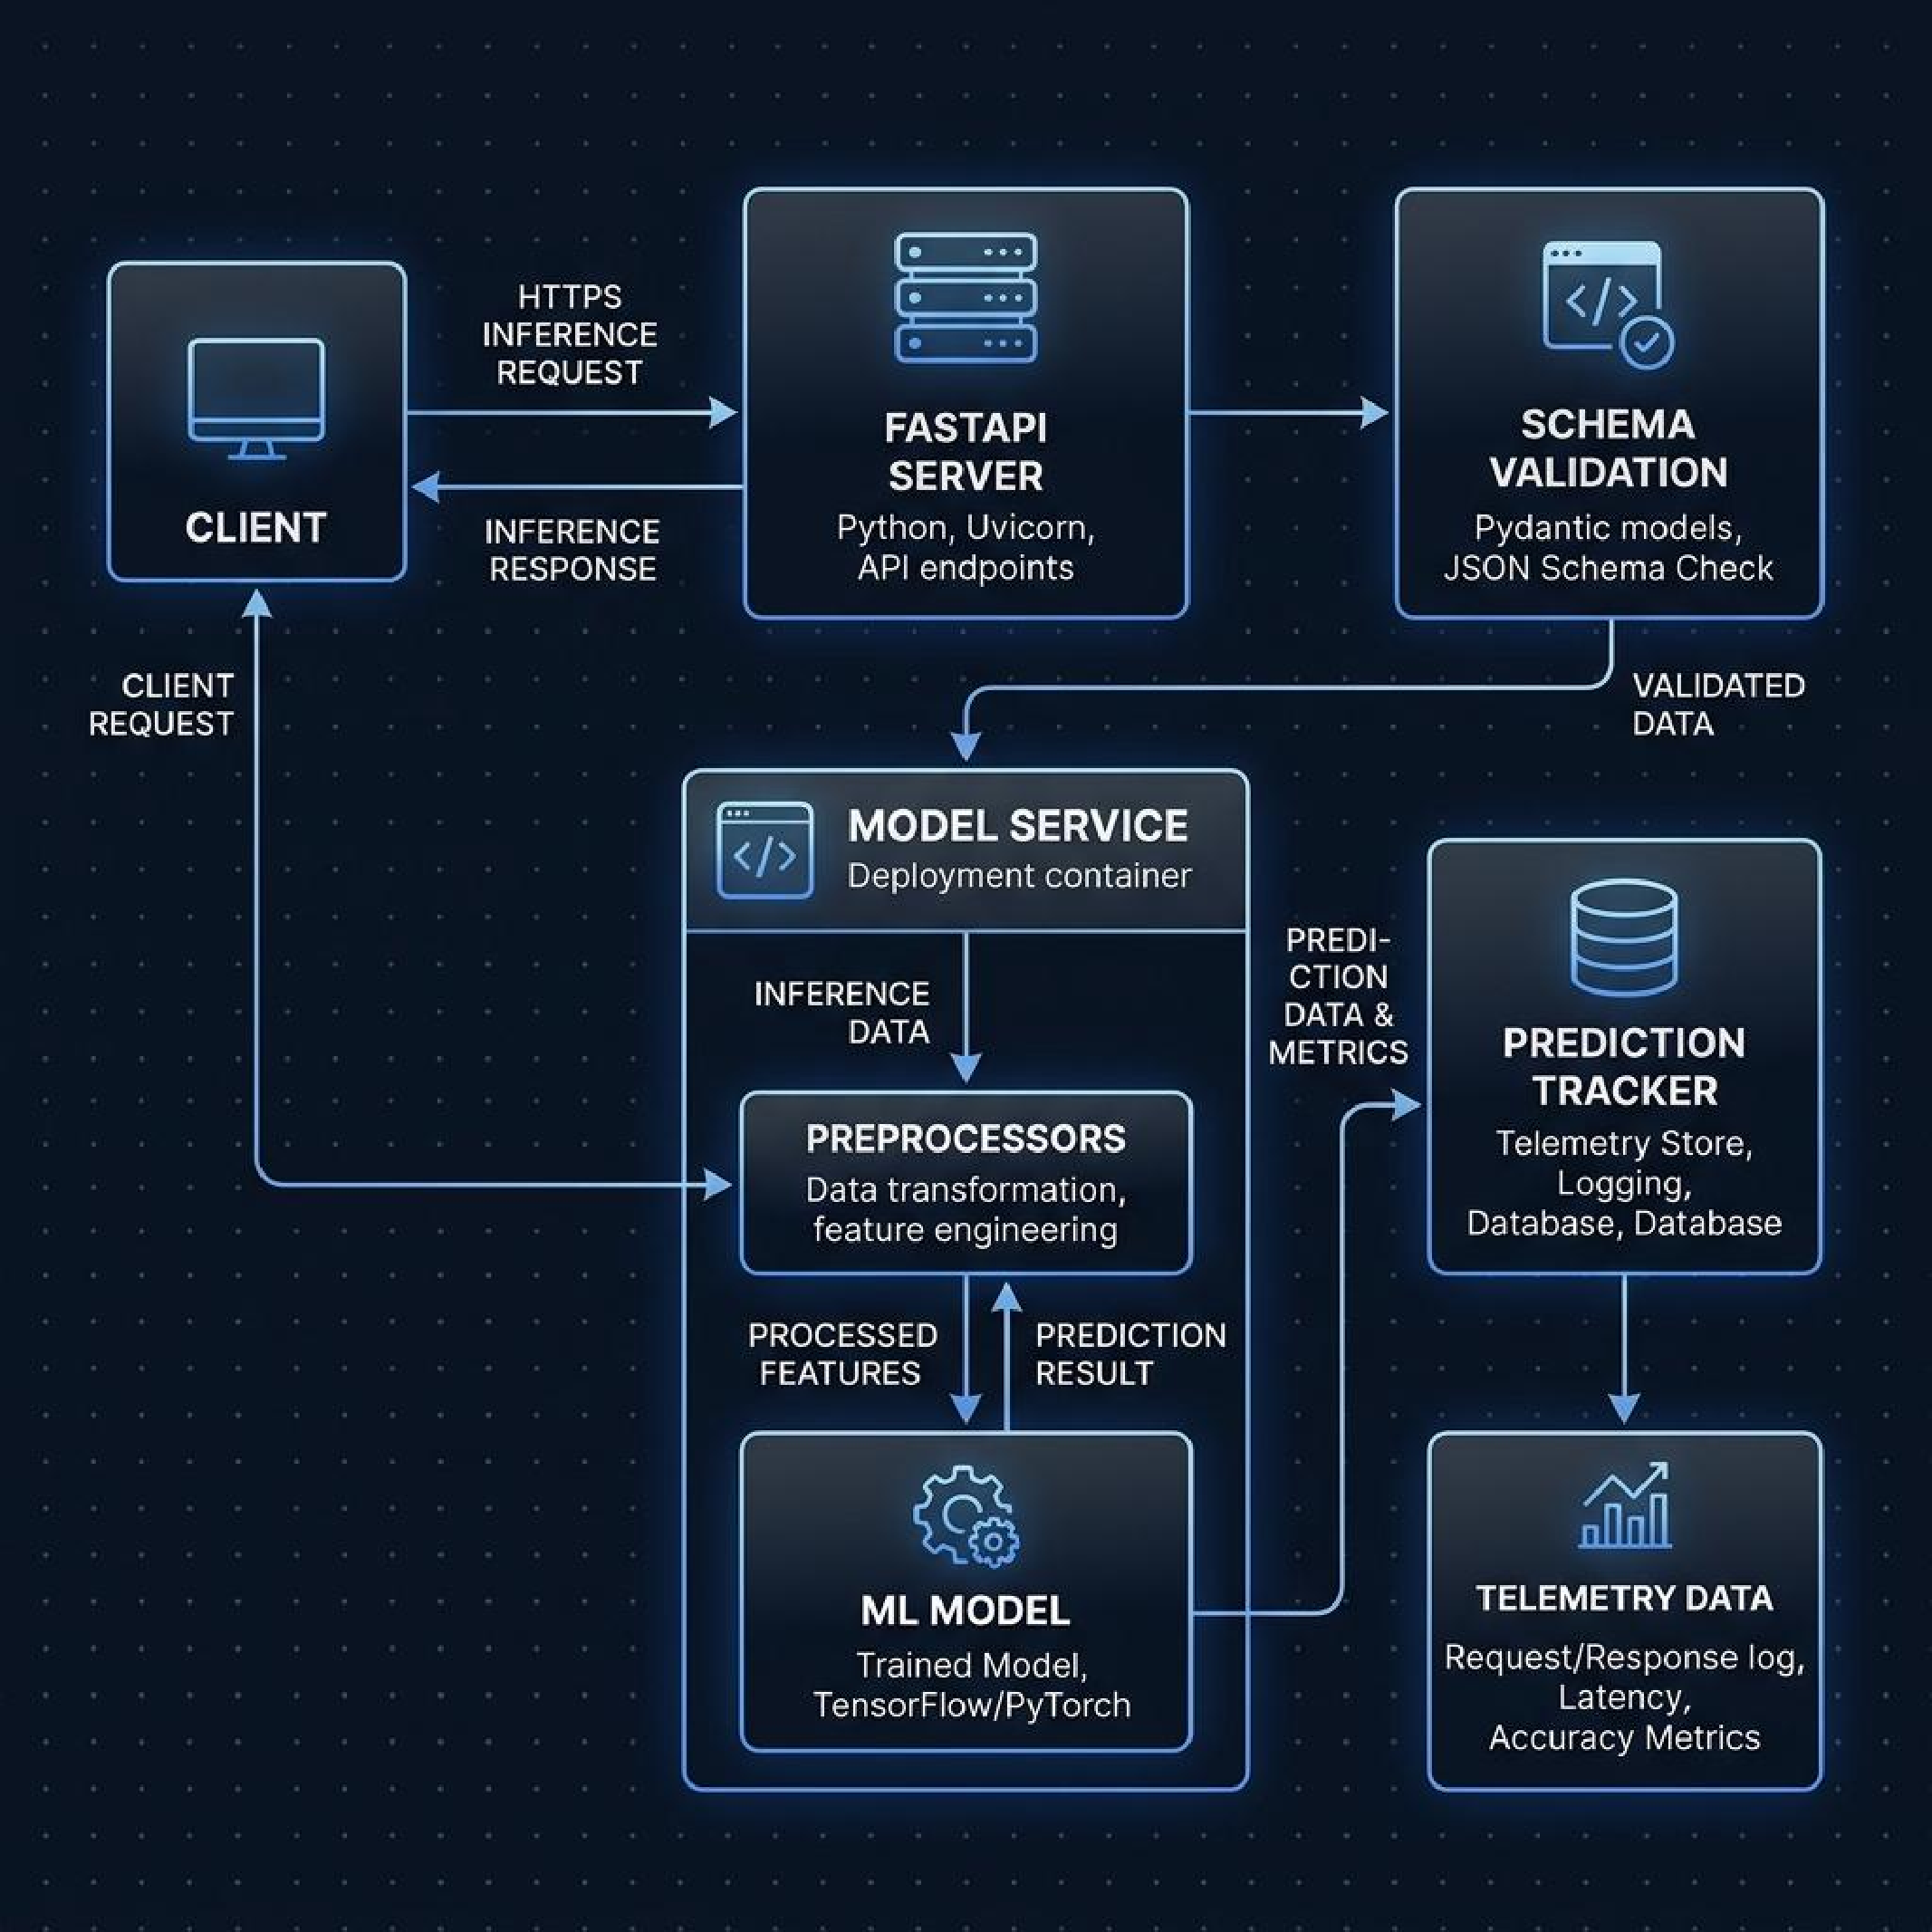
\includegraphics[width=0.85\textwidth]{../imgs/serving_architecture.pdf}
\caption{Model Serving and Validation Architecture}
\label{fig:serving_architecture}
\end{figure}

The system design relies on four core elements:
\begin{itemize}[leftmargin=*]
    \item \textbf{FastAPI Server:} Exposes standard inference endpoints for JSON payloads and batch inference endpoints for uploaded CSV files.
    \item \textbf{Great Expectations Schema Validation:} Validates incoming request values against expected bounds, preventing invalid inputs from reaching the model.
    \item \textbf{Telemetry Tracking:} Logs request inputs, outputs, timestamps, and execution times asynchronously to a JSON lines file on disk.
    \item \textbf{Model Version Control (VCS):} Creates unique commits of configuration and model binaries, allowing rollbacks to older deployments.
\end{itemize}

% -----------------------------------------------------------------------------
% CHAPTER 4: IMPLEMENTATION DETAILS
% -----------------------------------------------------------------------------
\chapter{Implementation Details}
\label{chap:methodology}

\section{Pipeline Module Parallel Scheduler}
The parallel scheduler in \systemname{} is implemented in C++ in \modulepath{src/core/graph.cpp}. When parallel execution is enabled, the graph uses \modulepath{std::async} to execute independent nodes concurrently. The scheduling logic uses counting semaphores to limit the number of active CPU threads, and a binary semaphore to serialize GPU access.

Algorithm~\ref{algo:run_parallel} shows the parallel execution logic. It tracks finished and started nodes, release the GIL during execution, and catches exceptions thrown by separate threads.

\begin{lstlisting}[style=algostyle,caption={Parallel Execution Engine in C++},label={algo:run_parallel}]
Input: execution_order nodes, cpu_threads limit
Output: executed graph with updated node states

1:   Release GIL via py::gil_scoped_release
2:   Initialize finished_executing map to false for all nodes
3:   Initialize started_executing map to false for all nodes
4:   Initialize CPU semaphore with cpu_threads count
5:   Initialize GPU semaphore with 1 (binary semaphore)
6:   Initialize atomic counter rem_nodes = size(execution_order)
7:   while rem_nodes > 0 do
8:       Acquire nodes semaphore
9:       for each node in execution_order do
10:          if started_executing[node] == true then continue
11:          check if all parent nodes are finished_executing
12:          if parents_finished == true then
13:              if node.uses_gpu == true then
14:                  Acquire GPU semaphore
15:              else
16:                  Acquire CPU semaphore
17:              end if
18:              set started_executing[node] = true
19:              spawn std::async(launch::async, [node]() {
20:                  Acquire GIL via py::gil_scoped_acquire
21:                  try {
22:                      node->execute()
23:                  } catch (...) {
24:                      store_exception()
25:                  }
26:                  decrement consumer counts for parent nodes
27:                  if parent consumer count == 0 then
28:                      release parent temporary memory
29:                  end if
30:                  set finished_executing[node] = true
31:                  decrement rem_nodes atomically
32:                  Release CPU/GPU semaphores
33:                  Release nodes semaphore
34:              })
35:          end if
36:      end for
37:  end while
38:  Re-throw any caught exceptions to the Python runtime
\end{lstlisting}

\subsection{Execution Flow and GIL Release Implementation}
The primary implementation challenge in the parallel execution flow was GIL (Global Interpreter Lock) contention. Because Python objects (such as scikit-learn estimators) are executed inside separate worker threads, concurrent calls will block each other if they attempt to manipulate Python references simultaneously. Mazen solved this by structuring a two-tier block wrapper in \modulepath{src/core/graph.cpp}:
\begin{enumerate}
    \item Before entering the loop-scheduling phase, the main thread releases the GIL using \texttt{py::gil\_scoped\_release}. This allows other native OS threads to run without waiting.
    \item Within each spawned worker thread, before invoking the node's \texttt{execute()} function, the GIL is explicitly acquired using \texttt{py::gil\_scoped\_acquire}. As soon as the call exits, the scope ends, immediately freeing the GIL for other concurrent threads.
\end{enumerate}

\subsection{Concurrency Semaphores and GPU Serialization}
To control the allocation of hardware resources, Mazen implemented custom semaphores using C++ synchronization primitives:
\begin{itemize}[leftmargin=*]
    \item \textbf{CPU Thread Limiter:} A counting semaphore initialized to \texttt{ACCELERA\_NUM\_THREADS} (or system cores minus one). Worker threads block on this semaphore before execution, preventing context-switching overhead from over-subscription.
    \item \textbf{GPU Access Lock:} A binary semaphore (mutex) used to serialize accesses to CUDA contexts. Because multiple threads submitting operations to the same GPU concurrently can cause driver crashes, any node with the \texttt{uses\_gpu} flag is forced to acquire this binary lock, serializing GPU execution while keeping CPU-bound preprocessing branches running in parallel.
\end{itemize}

\section{Merge Node and Voting Strategies}
The \modulepath{MergeNode} class combines outputs from multiple prediction branches. Mazen implemented this node in C++ (\modulepath{src/nodes/merge.cpp}) and connected it to NumPy and SciPy components. The node supports a hard-voting strategy implemented in C++:
\begin{itemize}[leftmargin=*]
    \item \textbf{Direct Class Predictions (1D Arrays):} Collects predicted category labels from all upstream branches, stacks them into a single 2D NumPy array (rows correspond to samples, columns to model outputs), and uses \modulepath{scipy.stats.mode} to extract the majority class label.
    \item \textbf{Probability Predictions (3D Arrays):} Stacks predicted probabilities across all branches. It computes class labels for each model using \texttt{np.argmax} across the probability dimensions and then applies majority voting on the resulting class labels.
\end{itemize}

\subsection{Voting Strategy Implementation and Edge Cases}
In \modulepath{src/nodes/merge.cpp}, Mazen handled several implementation edge cases:
\begin{enumerate}
    \item \textbf{Single-Model Fallback:} If the merge node only receives a single input branch, it directly routes the input to the output without calling voting functions, avoiding unnecessary computation.
    \item \textbf{Tie-Breaking:} When the voting results are split evenly, the node falls back to selecting the output of the first model (the primary branch), guaranteeing deterministic results.
    \item \textbf{GIL Safety in Numpy Stack:} Because stack operations call back into the Python/NumPy interpreter, the merge execution block is wrapped in a GIL acquisition scope, securing memory allocations.
\end{enumerate}

\section{Benchmark REST APIs and Dashboards}
Mazen designed and built the full client-server subsystem for the Benchmark module.

\subsection{Secure Backend Authentication Routes}
Implemented in Express and MongoDB in \modulepath{benchmark/backend/routes/user.js}:
\begin{itemize}[leftmargin=*]
    \item \textbf{Login Route (\texttt{POST /login}):} Sanitizes the input email, locates the user document, and compares the password against the stored bcrypt hash. Upon matching, it generates a signed JSON Web Token (JWT) with a 7-day expiration containing the user's MongoDB ID and role payload.
    \item \textbf{Signup Route (\texttt{POST /signup}):} Hashes new user passwords using a salt work factor of 10. If the email matches the environment parameter \texttt{ADMIN\_EMAIL}, the server automatically promotes the role to \texttt{"admin"}.
    \item \textbf{Deletion Route (\texttt{DELETE /:id}):} Restricted to admin users, allowing the deletion of any user profile except their own to prevent lockout.
\end{itemize}

\subsection{Submission Processing and Score Validation Route}
Implemented in \modulepath{benchmark/backend/routes/submissions.js}, the scoring route runs the evaluation pipeline when a user submits a CSV file:
\begin{enumerate}
    \item Downloader modules download the predictions CSV file and the hidden ground truth CSV from Google Drive.
    \item The backend validates the integrity of the files, verifying that the number of rows matches.
    \item It executes a Python worker subprocess configured with the target metric schema (e.g. F1-score or Mean Squared Error), calculates the performance score, and saves the submission to MongoDB.
\end{enumerate}

\subsection{Frontend Dashboards}
Built in React (\modulepath{benchmark/frontend/src/components/}) using state Hooks and async fetch requests:
\begin{itemize}[leftmargin=*]
    \item \textbf{User Dashboard (\texttt{dashboard.jsx}):} Displays a user's details, lists all benchmarks created by the user, and presents a grid of their submissions with performance scores and date history.
    \item \textbf{Admin Dashboard (\texttt{adminDashboard.jsx}):} Renders user lists and provides interactive deletion controls, checking JWT payloads to ensure administrative access.
\end{itemize}

\section{Deployment Module serving and Validation}
Mazen was fully responsible for implementing the Deployment module, which converts trained pipelines into containerized web services.

\subsection{Model Serving Subsystem}
\noindent Model serving is built on FastAPI and Uvicorn to handle concurrent HTTP requests. The subsystem loads the model and preprocessors via \texttt{ModelService}, which inspects the configuration (\texttt{config.json}) to locate the serialized artifacts. During execution, it runs input data through any fitted preprocessors in sequence before invoking the model's prediction method. A web-based graphical user interface (GUI) is dynamically rendered based on the expected input features, allowing users to submit single predictions interactively.

\noindent The following methods and files implement the serving logic:
\begin{itemize}[leftmargin=*]
  \item \modulepath{modelservice.py}:
    \begin{itemize}
      \item \texttt{ModelService.load()}: Parses \texttt{config.json} to discover the active model configuration. It opens and loads the main estimator file (e.g. \texttt{model.pkl}) and any auxiliary preprocessors (e.g. scalers or encoders) from the models directory.
      \item \texttt{ModelService.predict(input\_data, validate=True)}: Performs prediction. If validation is active, it calls \texttt{validate\_input(input\_data)} to receive validated and coerced values, converts the inputs into a NumPy array, adjusts dimensions, applies all loaded preprocessor transforms sequentially, and calls the underlying estimator's \texttt{predict()} method.
    \end{itemize}
  \item \modulepath{server.py}:
    \begin{itemize}
      \item \texttt{\_predict(input\_data, endpoint, filename=None)}: Coordinates serving telemetry. It records starting timestamps using \texttt{time.perf\_counter()}, executes model prediction via \texttt{ModelService.predict()}, calculates API response latencies, and logs metrics to the telemetry storage.
      \item \texttt{/predict} and \texttt{/predict/csv} Endpoints: Standard HTTP POST methods. The first endpoint receives a structured JSON payload, while the second parses uploaded CSV files into Pandas DataFrames.
      \item \texttt{/gui} and \texttt{/health} Endpoints: The GUI endpoint returns the dynamic interactive testing form via \texttt{\_render\_gui(schema)}, while the health endpoint serves load balancers with standard status checks.
    \end{itemize}
\end{itemize}

\subsection{Runtime Schema Validation}
\noindent To prevent invalid inputs from causing model crashes or silent degradation, incoming payloads are validated against a schema specified in the configuration. The validation layer uses Great Expectations to construct an ephemeral data source context. Columns are validated for expected names, missing entries, unexpected inputs, and value bounds (e.g., minimum and maximum thresholds). Data types are coerced automatically (e.g., matching string, boolean, integer, or floating-point formats) to match the training format, raising a structured \texttt{SchemaValidationError} if coercion fails.

\noindent The schema validation system is implemented in \modulepath{schema\_validation.py}:
\begin{itemize}[leftmargin=*]
  \item \texttt{InputSchema.\_\_init\_\_(config)}: Extracts features and limits from the configuration. If schema validation is enabled, it requests a Great Expectations context (\texttt{gx.get\_context()}), generates a unique UUID-based data source, registers a pandas-based DataFrame data asset, and configures a whole-dataframe batch definition.
  \item \texttt{InputSchema.validate(input\_data)}: Normalizes the input payload into a DataFrame. It checks for expected column presence, detects extra or missing features, runs the Great Expectations expectation suite, and executes type coercion.
  \item \texttt{InputSchema.coerce\_columns(df, errors)}: Loops through features to coerce types. It casts strings to numerical columns using \texttt{pd.to\_numeric(..., errors='coerce')}, checks for integer constraints (\texttt{value \% 1 == 0}), and processes boolean symbols (such as replacing \texttt{"true"}/\texttt{"false"} with Python booleans).
  \item \texttt{InputSchema.to\_dataframe(input\_data)}: Utility method to convert list, dict, or DataFrame structures into standard Pandas format.
\end{itemize}

\subsection{Telemetry and Request Tracking}
\noindent Production deployments capture inference requests and runtime metrics using a lightweight tracking layer. When enabled, the tracker logs prediction inputs, model outputs, processing latencies (measured in milliseconds), and timestamps. To avoid performance degradation on the prediction path, logging is written incrementally to a JSON lines (\texttt{.jsonl}) file.

\noindent Telemetry tracking is implemented in \modulepath{tracking.py}:
\begin{itemize}[leftmargin=*]
  \item \texttt{PredictionTracker.\_\_init\_\_(config)}: Sets up the file system paths and creates/opens the telemetry log file.
  \item \texttt{PredictionTracker.log\_prediction(inputs, outputs, latency, status)}: Formats request parameters, response targets, server latency, and datetime strings into a single-line JSON string and appends it to the logging stream.
\end{itemize}

\section{Multi-Target Deployment Orchestration}
\noindent The orchestration engine automates containerizing and launching the service across three distinct environments. It stages the codebase, copies project dependency requirements, and builds dockerized containers to ensure portability and reproducibility across platforms.
\begin{enumerate}[leftmargin=*]
  \item \textbf{Local Docker}: Generates a clean \texttt{Dockerfile} using a Python slim base image, stops any conflicting containers on the target port, builds the container image locally, and runs it.
  \item \textbf{Heroku}: Authenticates with the Heroku CLI and pushes/releases the Docker container using Heroku's Container Registry.
  \item \textbf{AWS EC2}: Creates an SSH transport connection and synchronizes the staging directory to the target host using \texttt{rsync} (excluding Python cache directories). It installs and starts the Docker daemon, builds the container on the instance, and executes local health check probes before verifying the public web endpoint.
\end{enumerate}

\begin{figure}[H]
\centering
\makebox[\textwidth][c]{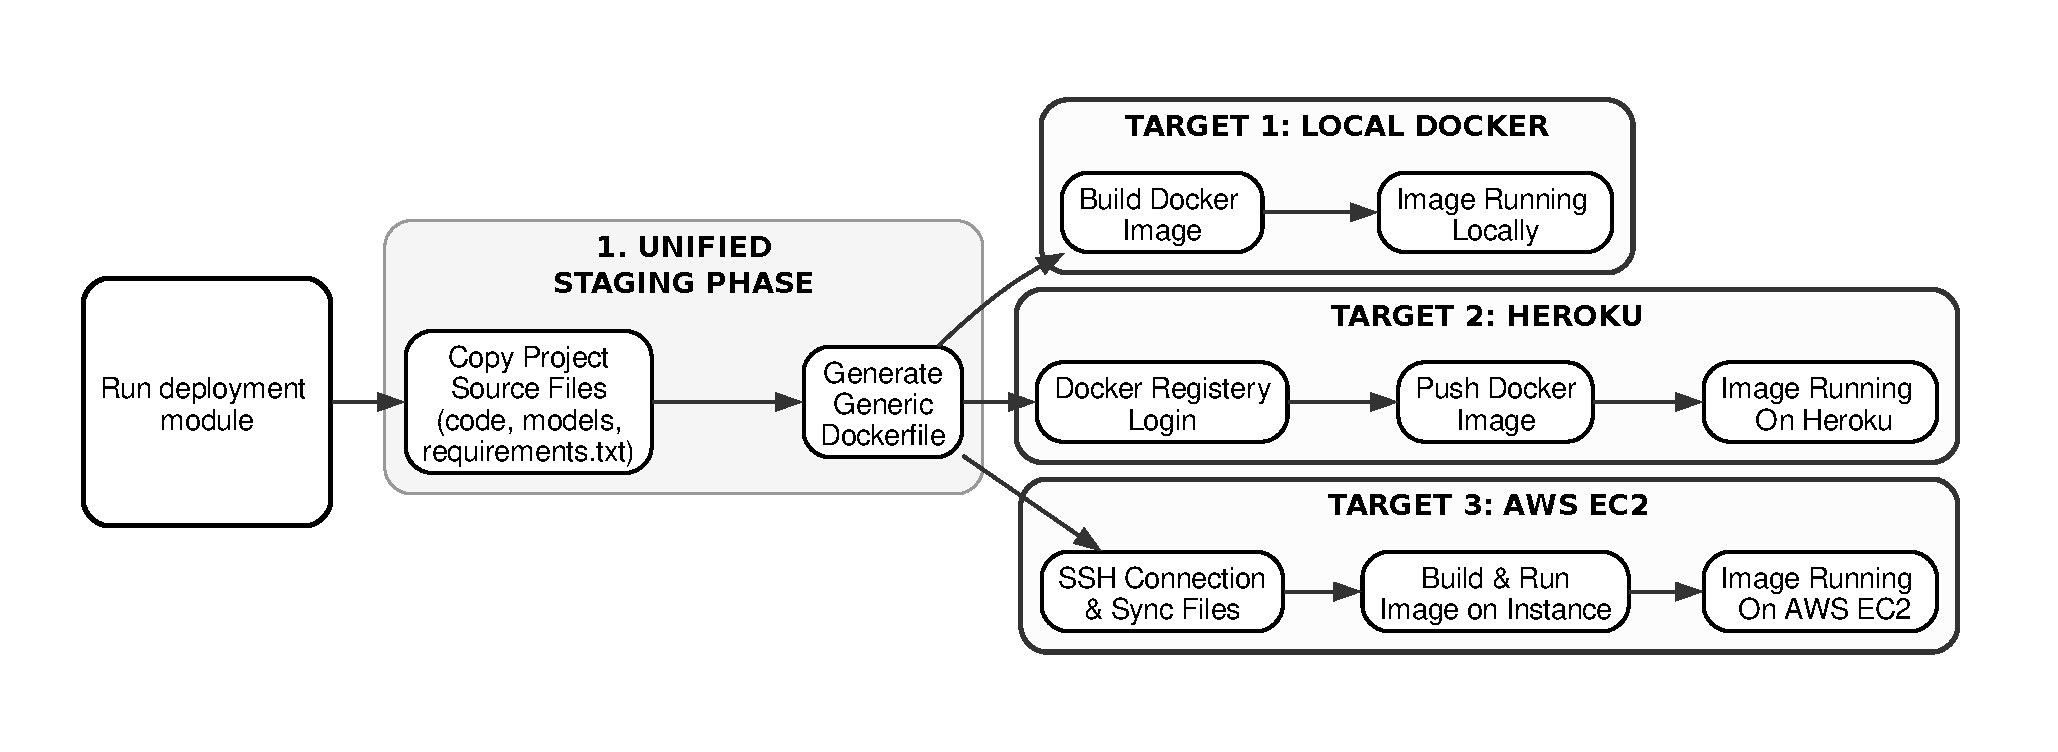
\includegraphics[width=1.2\textwidth]{../dots/deployment_targets.pdf}}
\caption{Deployment Orchestration Workflow}
\label{fig:orchestration_flow}
\end{figure}

\section{Model Version Control (VCS)}
\noindent The internal VCS provides reproducibility for deployed pipelines. It calculates a stable SHA-1 hash for each commit based on its timestamp and commit message. Models and configurations are archived into an \texttt{experiments/} subdirectory. The system maintains a global index (\texttt{experiments.json}) containing parent-child commit histories, HEAD references, and active deployed markers, facilitating rollbacks and deployments of historical model versions.

\noindent The version control subsystem is implemented in \modulepath{vcs.py}:
\begin{itemize}[leftmargin=*]
  \item \texttt{calculate\_hash(timestamp, message)}: Computes the 7-character SHA-1 hash value that acts as the commit identifier.
  \item \texttt{init(args)}: Configures the repository workspace by creating directories and saving the default index (\texttt{experiments.json}).
  \item \texttt{commit(args)}: Validates that models exist, generates a commit hash, copies the active configuration and models to \texttt{experiments/<hash>/}, and appends the commit entry to the registry.
  \item \texttt{log(args)}: Lists all recorded commits, showing details such as commit hash, creation date, message, and deploy status.
  \item \texttt{show(args)}: Displays the details and settings of a target commit.
  \item \texttt{deploy(args)}: Deploys a specific commit by copying its stored model files and configuration back into the active runtime workspace.
\end{itemize}

\begin{figure}[H]
\centering
\makebox[\textwidth][c]{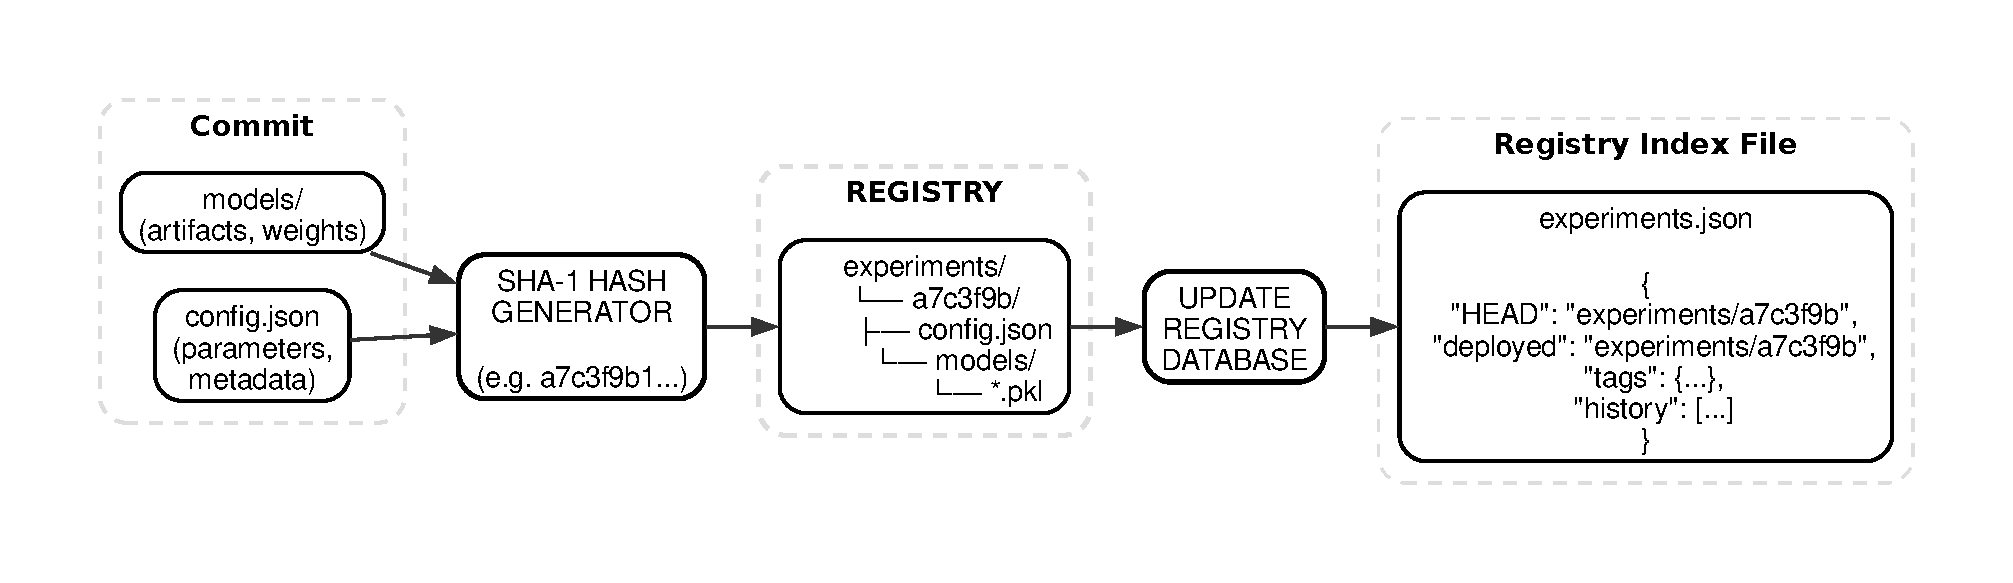
\includegraphics[width=1.2\textwidth]{../dots/deployment_commit.pdf}}
\caption{VCS Commit Workflow}
\label{fig:vcs_commit_flow}
\end{figure}

\begin{figure}[H]
\centering
\makebox[\textwidth][c]{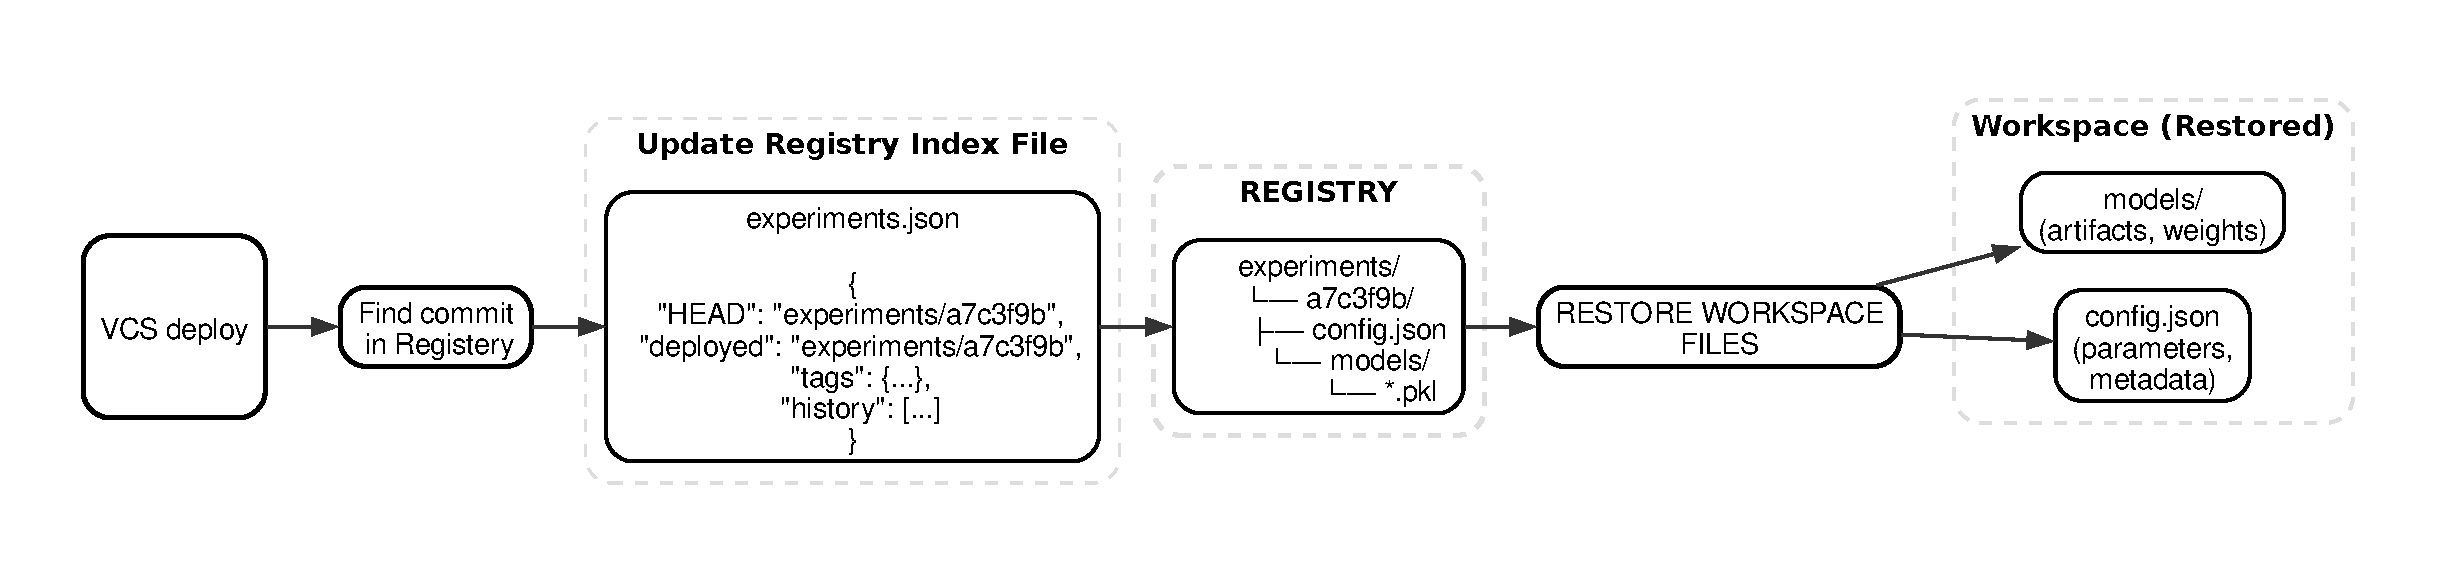
\includegraphics[width=1.2\textwidth]{../dots/deployment_deploy.pdf}}
\caption{VCS Deploy Workflow}
\label{fig:vcs_deploy_flow}
\end{figure}

\section{Command-Line Interface and CLI Commands}
\noindent The orchestrator and version control features are exposed to the user through command-line interfaces inside \modulepath{deployment.py} and \modulepath{vcs.py}. The supported commands and their behaviors are:

\subsubsection{Orchestrator Commands}
\begin{itemize}[leftmargin=*]
  \item \textbf{prepare}: Prepares the deployment staging area. It copies service modules (e.g. \texttt{server.py}, \texttt{modelservice.py}) and the \texttt{accelera} source library to the \texttt{accelera\_deployment} folder, and generates the serving \texttt{Dockerfile} and \texttt{requirements.txt}.
  \item \textbf{build}: Builds the local Docker container. It invokes local subprocess shell commands (e.g. \texttt{docker build -t <image\_name> .}) with an optional \texttt{--no-cache} flag.
  \item \textbf{run-local}: Starts the local Docker container. It stops and removes any conflicting containers on the port before launching the container using port mappings.
  \item \textbf{local}: Orchestrates the complete local container pipeline by sequentially running the \textbf{prepare}, \textbf{build}, and \textbf{run-local} steps.
  \item \textbf{heroku-login}: Logs the client environment into the Heroku CLI and Heroku Docker registry.
  \item \textbf{heroku-deploy}: Packages and deploys the container to Heroku. It triggers login, pushes the Docker image to Heroku's registry, and releases the container for traffic.
  \item \textbf{heroku-push} and \textbf{heroku-release}: Granular command calls that push the container image and release it separately.
  \item \textbf{ec2-deploy}: Deploys to a remote AWS EC2 instance. It establishes an SSH connection, synchronizes files using \texttt{rsync}, compiles/builds the Docker container on the host, runs it, and probes local health targets.
  \item \textbf{ec2-status}, \textbf{ec2-logs}, and \textbf{ec2-stop}: Operational tools to verify container execution, read Uvicorn outputs, and terminate the container on the target EC2 node.
\end{itemize}

\subsubsection{Version Control Commands}
\begin{itemize}[leftmargin=*]
  \item \textbf{init}: Sets up a new model version control workspace by initializing directories and registries.
  \item \textbf{commit}: Snapshots active model parameters and configurations under a message flag (\texttt{-m}).
  \item \textbf{log}: Prints the history log of all model commits.
  \item \textbf{show}: Prints the configuration dictionary details of a target commit.
  \item \textbf{deploy}: Restores a specified commit back into the staging area for subsequent deployment execution.
\end{itemize}

\section{Design Constraints and Challenges}
\noindent The design of the Deployment module is subject to several key constraints:
\begin{itemize}[leftmargin=*]
  \item \textbf{Package Size Optimization}: To minimize container build times and storage footprints, heavy libraries like PyTorch or TensorFlow are excluded from the serving runtime unless explicitly required by the model.
  \item \textbf{Non-Interactive Execution}: Staging and EC2 orchestration must run headlessly in CI/CD pipelines, necessitating automatic Docker installs and automated SSH host key acceptance (\texttt{StrictHostKeyChecking=accept-new}).
  \item \textbf{I/O Isolation}: Process and SSH connection errors are caught as base \texttt{OSError} types to provide descriptive feedback on firewall and network issues without interrupting local execution.
\end{itemize}

During development, Mazen addressed three major implementation challenges:
\begin{enumerate}
    \item \textbf{Great Expectations Init Latency:} Creating the GX validation context on every request inflated latencies by ~1.2 seconds. Mazen solved this by instantiating the context only once during class initialization in \modulepath{InputSchema} and validating incoming payloads in memory.
    \item \textbf{EC2 Port Binding Lockups:} SSH commands occasionally hung if the remote port was bound to a zombie process. Mazen resolved this by adding a pre-flight cleaning command (\texttt{fuser -k -n tcp <port>}) to force-release the target port before running the Docker container.
    \item \textbf{Asynchronous Logging Race Conditions:} High-frequency concurrent requests caused line fragmentation in the telemetry logging file. Mazen resolved this by wrapping the write calls in an append loop using Python file locking (\modulepath{fcntl.flock}), ensuring write atomicity.
\end{enumerate}

% -----------------------------------------------------------------------------
% CHAPTER 5: SYSTEM TESTING AND VERIFICATION
% -----------------------------------------------------------------------------
\chapter{System Testing and Verification}
\label{chap:verification}

\section{Pipeline Verification}
The parallel executor and voting strategies were verified using unit tests.
\begin{itemize}[leftmargin=*]
    \item \textbf{Parallel Execution Tests:} Verify that the topological execution order is preserved, independent branches execute concurrently, and GIL lock release/acquisition behaves correctly.
    \item \textbf{Merge Node Tests:} Validate the correctness of the C++ hard-voting implementation. The test cases verify that the argmax voting correctly matches SciPy baselines for 1D and 3D prediction arrays, and handles the single-model edge case.
\end{itemize}

\section{Benchmark Subsystem Verification}
The benchmark module tests check that the Node.js API endpoints and database operations behave correctly:
\begin{itemize}[leftmargin=*]
    \item \textbf{Authentication tests:} Check token generation, verify that invalid login details are rejected, and confirm that the signup route hashes passwords correctly.
    \item \textbf{Dashboard routing tests:} Validate user-dashboard calls and verify that admin-level routes reject normal user accounts.
    \item \textbf{Validation tests:} Verify that the server rejects submissions with incorrect row counts or invalid URL structures.
\end{itemize}

\section{Deployment Module Verification}
\noindent The verification of the Deployment module is performed through a comprehensive test suite managed by the \texttt{pytest} framework. To ensure high test isolation and allow headless execution in CI/CD pipelines, the test suite leverages extensive mocking via the Python \texttt{monkeypatch} utility to decouple tests from system-level configurations, active network services (e.g., Heroku API, AWS EC2 hosts), and runtime dependency installations. 

\noindent Tests are executed inside temporary filesystem workspaces generated dynamically using the \texttt{tmp\_path} fixture. This ensures that the generated version control indices, log files, and Docker deployment artifacts do not contaminate the primary workspace.

\subsection{Subsystem Verification Details}
\noindent The verification targets the six major components of the deployment module:

\begin{enumerate}[leftmargin=*]
  \item \textbf{Model Version Control (VCS) verification}:
    Validates the stability of the 7-character short SHA-1 hash calculation, confirming that identical timestamp-message pairs produce identical commit IDs. Tests ensure that \texttt{vcs.init()} initializes the experiments metadata directory structure and saves a clean registry template (\texttt{experiments.json}). Commit operations are verified to correctly copy model serialization binaries (e.g., \texttt{model.pkl}), snapshot active configurations, update the \texttt{HEAD} reference, and append metadata entries. Rollback capabilities are verified by deploying historical commits and confirming that the active runtime files are updated with the corresponding commit snapshots.
  
  \item \textbf{Model Service Pipeline verification}:
    Tests check that the \texttt{ModelService} correctly parses configurations, loads active model estimators and preprocessors in the correct sequence, and performs inference. Mock tests confirm that preprocessing steps (such as scaling or encoding) are applied in order before predictions are generated.
  
  \item \textbf{Runtime Schema Validation verification}:
    Validates the runtime behavior of input schema checking. Ephemeral Great Expectations suites are mocked to verify column-presence verification (identifying missing or unexpected fields) and value-bound checking. The data type auto-coercion system is verified by testing how it handles numeric conversions (casting strings to floats or integers) and parsing boolean representations (such as \texttt{"true"}, \texttt{"false"}, or numeric binary flags).
  
  \item \textbf{Web Serving Endpoints verification}:
    Verifies that the FastAPI application correctly routes incoming HTTP requests. Tests evaluate the \texttt{/predict} and \texttt{/predict/csv} endpoints for JSON inputs and multi-row CSV file uploads. Endpoint testing checks that success responses return correct JSON structures with HTTP 200 codes, validation errors throw HTTP 422 codes, and server errors return HTTP 500 codes.
  
  \item \textbf{Prediction Tracking and Telemetry verification}:
    Verifies the telemetry logging behavior. Tests ensure that when telemetry is disabled, no disk writes occur. When active, request parameters, model outputs, timestamps, and latency figures are verified to be written as valid JSON lines to the log file. Additionally, tests verify the telemetry reader's ability to aggregate counts (successful runs, error runs, total row counts) and report them dynamically.
  
  \item \textbf{Orchestration CLI verification}:
    Validates port parsing limits (allowing ports between 1 and 65535, while rejecting negative numbers, non-numeric values, or out-of-bound ports). Tests check the preparation task (\texttt{prepare}) to verify that it creates a clean staging directory, compiles a standard \texttt{Dockerfile} using a Python slim base, and builds a clean \texttt{requirements.txt} containing only runtime-specific dependencies.
\end{enumerate}

\subsection{Deployment Test Results}
\noindent When executed in an environment with all core dependencies installed, all 51 test cases compile and pass successfully. Table~\ref{tab:deployment-test-summary} summarizes the verification results for the deployment module.

\begin{table}[H]
\centering
\caption{Deployment Module Test Suite Verification Summary}
\label{tab:deployment-test-summary}
\begin{tabular}{lrrrl}
\toprule
\textbf{Test Component File} & \textbf{Test Cases} & \textbf{Passed} & \textbf{Failed} & \textbf{Verified Feature} \\
\midrule
\texttt{vcs\_test.py} & 14 & 14 & 0 & Registry snapshots, workspace rollbacks \\
\texttt{modelservice\_test.py} & 6 & 6 & 0 & Sequencing of preprocessor transforms \\
\texttt{schema\_validation\_test.py} & 8 & 8 & 0 & Data coercion and column checking \\
\texttt{server\_test.py} & 9 & 9 & 0 & FastAPI routing, telemetry integration \\
\texttt{tracking\_test.py} & 3 & 3 & 0 & Telemetry logging and count aggregation \\
\texttt{deployment\_test.py} & 11 & 11 & 0 & Staging setup, Dockerfile compiling \\
\midrule
\textbf{Total} & \textbf{51} & \textbf{51} & \textbf{0} & \textbf{End-to-End System Correctness} \\
\bottomrule
\end{tabular}
\end{table}

\noindent This successful validation confirms that the deployment engine operates as intended, offering robust models, automated runtime validation, telemetry logging, and repeatable container deployments without regression errors.

% -----------------------------------------------------------------------------
% CHAPTER 6: CONCLUSIONS AND FUTURE WORK
% -----------------------------------------------------------------------------
\chapter{Conclusions and Future Work}
\label{chap:conclusion}

\section{Summary of Contributions}
In this graduation project, Mazen Adel designed, implemented, and verified key subsystems for \systemname{}:
\begin{itemize}[leftmargin=*]
    \item \textbf{Pipeline Execution Layer:} A concurrent C++ scheduler utilizing semaphores for hardware thread limitation, safety gates for GPU tasks, and active consumer counting for memory release, paired with numpy/scipy-based majority voting nodes.
    \item \textbf{Benchmark Subsystem:} A Node.js Express backend and MongoDB schema model supporting JWT/bcrypt authentication and a React frontend for task management, dashboards, and leaderboard display.
    \item \textbf{Serving and Deployment Infrastructure:} A production-ready FastAPI model server featuring Great Expectations schema validation, async request tracking, model versioning (VCS) hash snapshotting, and automated scripts for Local Docker, Heroku, and remote AWS EC2 deployment targets.
\end{itemize}

\section{Future Extensions}
Future improvements can focus on the following:
\begin{itemize}[leftmargin=*]
    \item \textbf{Horizontal Scheduling:} Extend the pipeline parallel scheduler to distribute graph branches across different cluster nodes instead of limiting execution to a single host.
    \item \textbf{Robust Encryption:} Improve data security in the benchmark module by encrypting ground truth files on MongoDB and verifying predictions inside sandbox runners.
    \item \textbf{Serverless Serving Targets:} Add serverless deployment capabilities (such as AWS Lambda) to the orchestrator to deploy lightweight models without maintaining active virtual servers.
\end{itemize}

\end{document}
